\section{Úrovně detailu}
\label{sec-LOD}
V předchozích kapitolách předpokládáme zpracování a zobrazování geometrického modelu vegetace. Pro nižší úrovně detailu (LOD) lze využít metod, které složitou geometrii typicky nahrazují zobrazením primitivní geometrie (např. čtverce), na které je aplikována textura (obrázek) navozující dojem, že se jedná o původní objekt. Zaznamenáme-li pohledy na objekt z několika směrů, lze s určitou rozumnou tolerancí ke snížení kvality zobrazit následně pomocí těchto pohledů libovolný pohled na objekt bez nutnosti zobrazení a zpracování jeho plné geometrické reprezentace. Úspora potřebného výkonu spočívá jak v malém počtu zpracovávaných vrcholů geometrie, tak v ušetření řady rasterizačních operací stejně jako v menším počtu zpracovávaných fragmentů.
\footnote{ předpokládá se, že jednotlivé listy jsou vykreslovány v náhodném pořadí a tím pádem je barva určitého pixelu několikrát přepisována}
 Výsledná kvalita zobrazeného objektu je ovlivněna počtem předgenerovaných pohledů, jejich kvalitou a také způsobem, jak zkonstruovat obraz pro pohled ze směru, pro který neexistuje předgenerovaný obraz.
Známé jsou metody billboardingu využívající pro osově souměrnou geometrii jediného pohledu, který je natáčen kolmo k pohledu virtuální kamery. \footnote{existuje několik možností natáčení obrázku např:
\begin{itemize}
\item rovnoběžně se stínítkem kamery
\item kolmo k pohledu kamery
\end{itemize}
}
Relativně běžná je metoda využívající jakýchsi trsu billboardů. Objekt je nahrazen množinou různě orientovaných geometrických primitiv, jak je patrné z obrázku 
\begin{figure}[!hbt]
\begin{center}
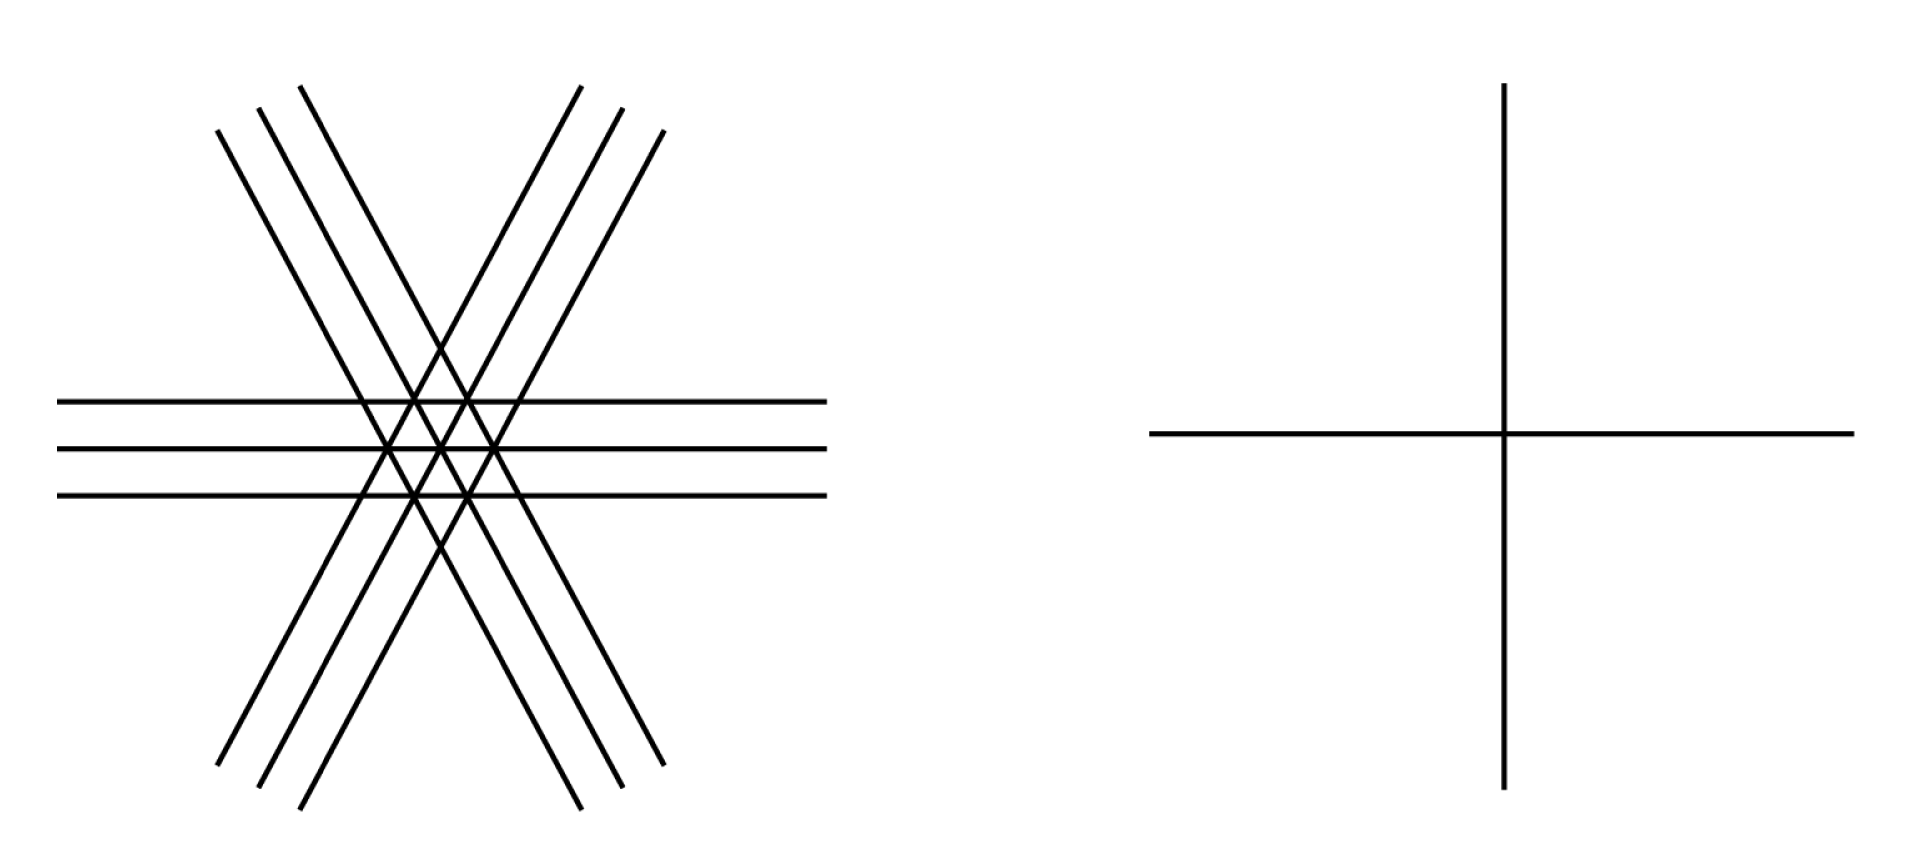
\includegraphics[width=0.75\textwidth]{./figures/slicesTop.png}
\caption[Konstrukce jednoduchého trsu billboardů]%
{ Konstrukce jednoduchého trsu billboardů: (pohled zvrchu) vyšší LOD tvořený třemi skupinami billboardů po 3 řezech (vlevo), nižší LOD tvořený pouze dvěma kolmými billboardy (vpravo) }
\end{center}
\label{fig:sliceBilboard}
\end{figure}

Na rozdíl od metod skutečného billboardingu, trsy billboardů si zachovávají svou orientaci vůči světovým souřadnicím ve scéně. Tento koncept lze vylepšit pro zobrazování objektů, jako jsou stromy tím, že přidáme další rovnoběžné billboardy. Struktura koruny stromu je dosti členitá a při pohybu kolem stromu se uplatňuje paralaxa a dochází k překrývání větví a listů. K tomu dochází i v případě pohybu samotného stromu. Budeme-li uvažovat v určitých částech průhledné obrázky použité v trsu rovnoběžných billboardů, pak lze podobných efektů docílit. Sadu rovnoběžných billboardů lze chápat jako různé řezy geometrií. Do každého řezu se promítne určité okolí tak, aby celkově všechny rovnoběžné řezy pokrývaly rovnoměrně celou původní geometrii. Řezy lze předgenerovat pro statický strom a používat je následně pro každou instanci daného stromu ve scéně. Předpokládá se rovněž, že v rámci jednoho řezu bude vytvořen soubor informací potřebný k pozdějšímu zobrazení a animaci (např. barevné, normálové a hloubkové mapy).
\begin{figure}[!hbt]
\begin{center}
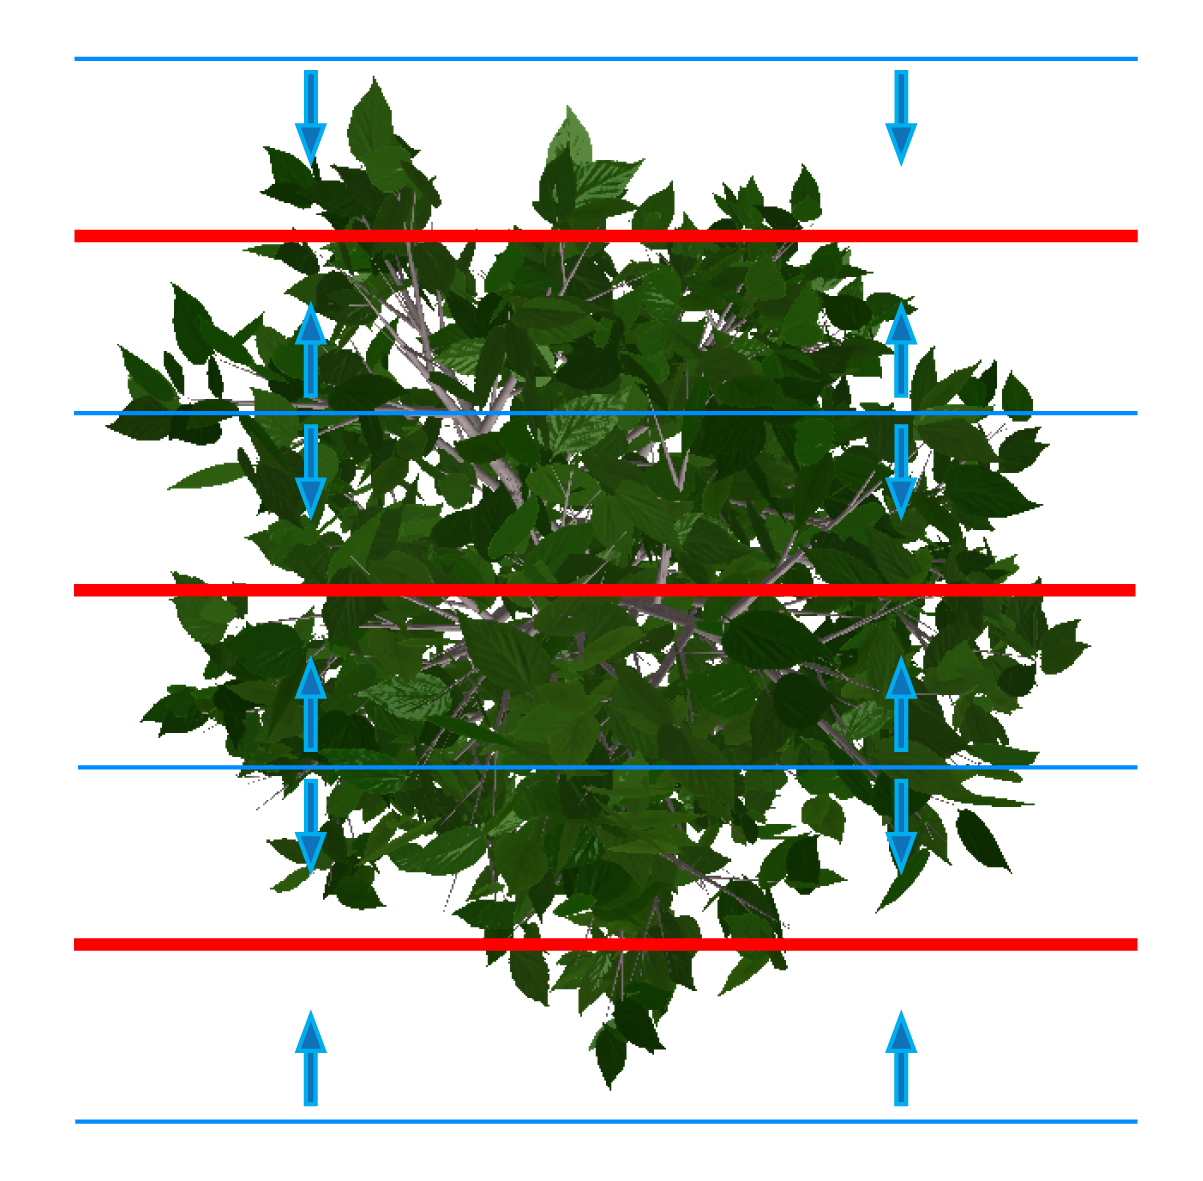
\includegraphics[width=0.5\textwidth]{./figures/slices.png}
\caption[Tvorba řezů pro vícevrstvé billboardy]%
{ Tvorba řezů pro vícevrstvé billboardy. Jednotlivé textury řezů jsou znázorněny červeně. }
\end{center}
\label{fig:slicing}
\end{figure}
Čím je objekt od pozorovatele vzdálenější, tím méně se tyto efekty uplatňují a tím menší má objekt percepční váhu, proto lze v rámci zvýšení výkonu snižovat počet obrázků (textur) v trsu.
Protože se orientace trsu řezů vůči scéně nemění, mohou vznikat nepříjemné artefakty tím, že směr pohledu bude téměř rovnoběžný s rovinou některého z řezů. Z toho důvodu je dobré zajistit, aby se takové řezy vůbec nezobrazovaly. 

Pro velmi vzdálené stromy se již neprojevuje efekt paralaxy skoro vůbec a pozorovatel vnímá pouze tvar obrysu stromu a jeho celkovou barevnost. Z toho důvodu lze tyto velmi vzdálené stromy nahradit zjednodušenou verzí LOD, která je představována pouze dvěma navzájem kolmými řezy.  


\subsection{Animace v image-base modelu}
\label{sec-ibAnimation}

Bohužel z povahy konstrukce trsu řezů dochází ke ztrátě velikého množství informací, které jsou podstatné pro provedení animace v rozsahu a kvalitě odpovídající postupu popsaného v kapitole \ref{sec-animation3D}. Větve jsou většinou zakryty listy. Jednotlivé listy se také překrývají a tak například o listech, které nejsou vidět nelze získat žádné informace. Naštěstí nemají modely zobrazené touto metodou vysokou percepční váhu (jde o nižší LOD) a lze si tudíž dovolit snížení kvality a přistoupit k animaci zcela jinak.
Základním předpokladem je, že deformace se provádí pouze v dvourozměrném prostoru textury jednoho řezu. Zatímco původní deformace je realizovatelná ve vertex shaderu, tento postup využije s výhodou možností fragment shaderu. Vyplývá z toho však nepříjemné omezení, které mění původní problém, který lze shrnout otázkou: \emph{„Kam se posune tento bod?“} (nazývejme {\bf přímá transformace}), na problém typu \emph{„Jaký bod se přesune do tohoto místa?“} (nazývejme {\bf zpětná transformace}). Fragment shader totiž neumožňuje měnit aktuálně zpracovávanému fragmentu pozici, na kterou bude zapsán ve výstupním bufferu. Uvážíme-li, že se na určitou pozici může po transformaci zobrazit i několik fragmentů, bylo by pro korektní zobrazení nutné projít každý texel textury provést přímou transformaci a zjistit, zda není dosaženo aktuální pozice. Takové řešení je ovšem značně nevhodné.

Jestliže je třeba provádět v rámci jediné textury různé transformace, které přísluší různým zobrazeným větvím, pak je třeba znát, jaká transformace se v daném bodě bude provádět. Musí být tedy předem jasné, jaká větev se do daného bodu může zobrazit. Současně s generováním textur pro jednotlivé řezy, je možné připravit i texturu, která bude tuto informaci obsahovat. Jednoduchým řešením, které lze i efektivně implementovat na GPU, je vytvoření oblastí, které odpovídají buňkám Voronoiova diagramu – tedy pro daný bod nalezneme nejbližší bod, kde je zobrazena větev ve výchozím stavu. Tento postup můžeme nazvat {\bf „propagace dat“}.

\begin{figure}[!hbt]
\label{fig:sliceBilboard}
\begin{center}
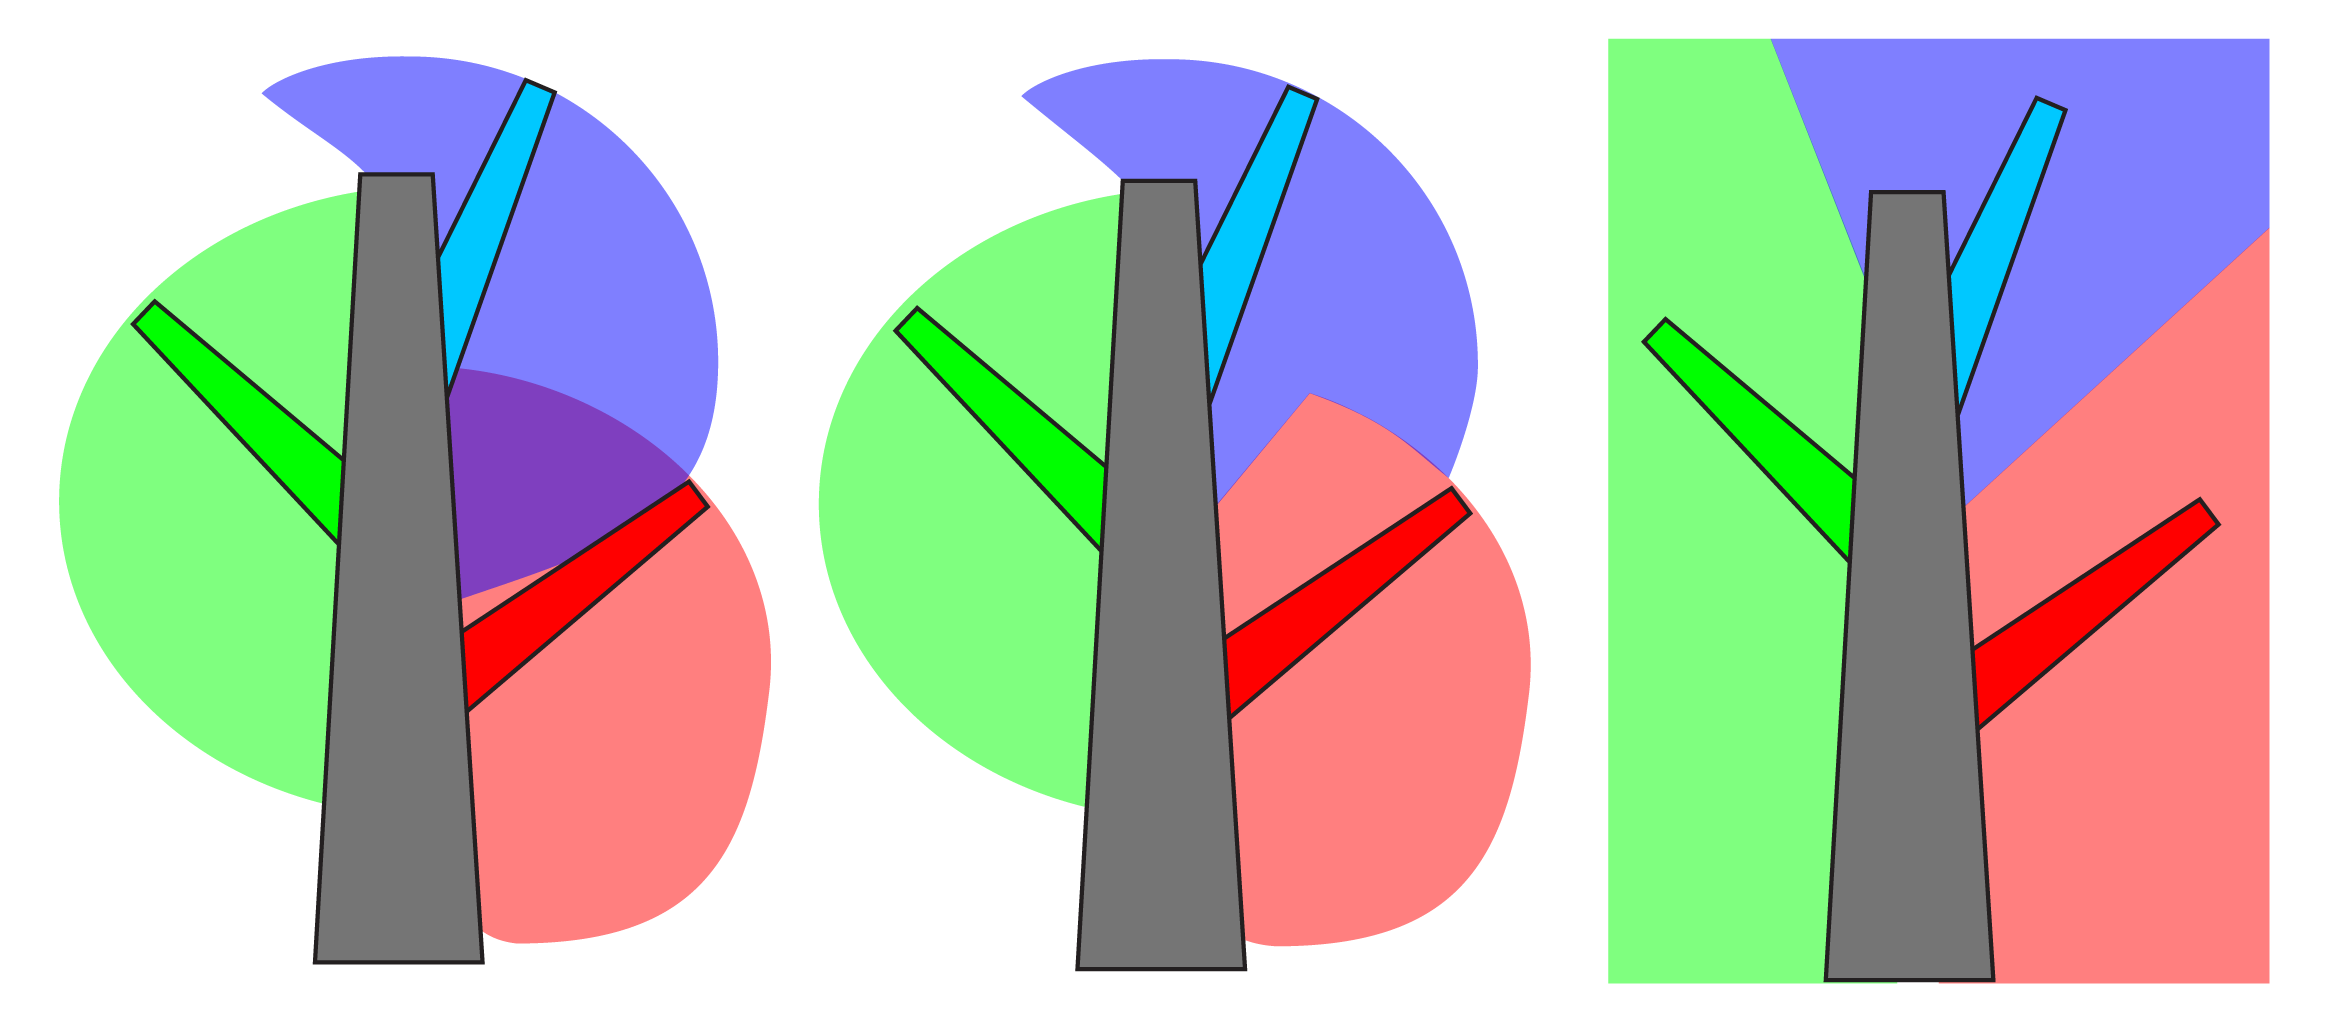
\includegraphics[width=0.75\textwidth]{./figures/dataExpansionPrinciple.png}
\caption[Schematicky znázorněné oblasti, kam se mohou větve deformovat]%
{Schematicky znázorněné oblasti, kam se mohou větve deformovat. Černě vytaženy obrysy výchozí polohy zobrazených větví
(vlevo) reálný ohyb – oblasti se překrývají, (uprostřed) oblasti bez překryvů, (vpravo) oblasti Voronoiova diagramu}
\end{center}
\end{figure}

Pokud tedy známe, jaká větev se může do daného bodu $P$ deformovat, známe také parametry této deformace. Z důvodů zachování koherence animace (větve se pohybují zhruba stejně) využijeme metodu deformace vycházející z ohybu trojrozměrného modelu. Trojrozměrný ohyb je prováděn v souřadném systému větve ($S_b$). Po převedení bázových vektorů ($\vec{r}_b$,$\vec{s}_b$,$\vec{t}_b$) do souřadného systému řezu ($S_p$ – tedy vektory $\vec{r}_p$,$\vec{s}_p$,$\vec{t}_p$) je možné postupovat prakticky stejně. Uplatníme myšlenkový model, kdy bod $P_0$ mimo větev (představovaná osou x) bude při deformaci udržovat svou relativní pozici na normále k větvi (viz obrázek \ref{fig:bendModel}). Potřebujeme tedy zjistit, ke kterému bodu větve je bod $P_p$ ukotven.

\begin{figure}[!hbt]
\begin{center}
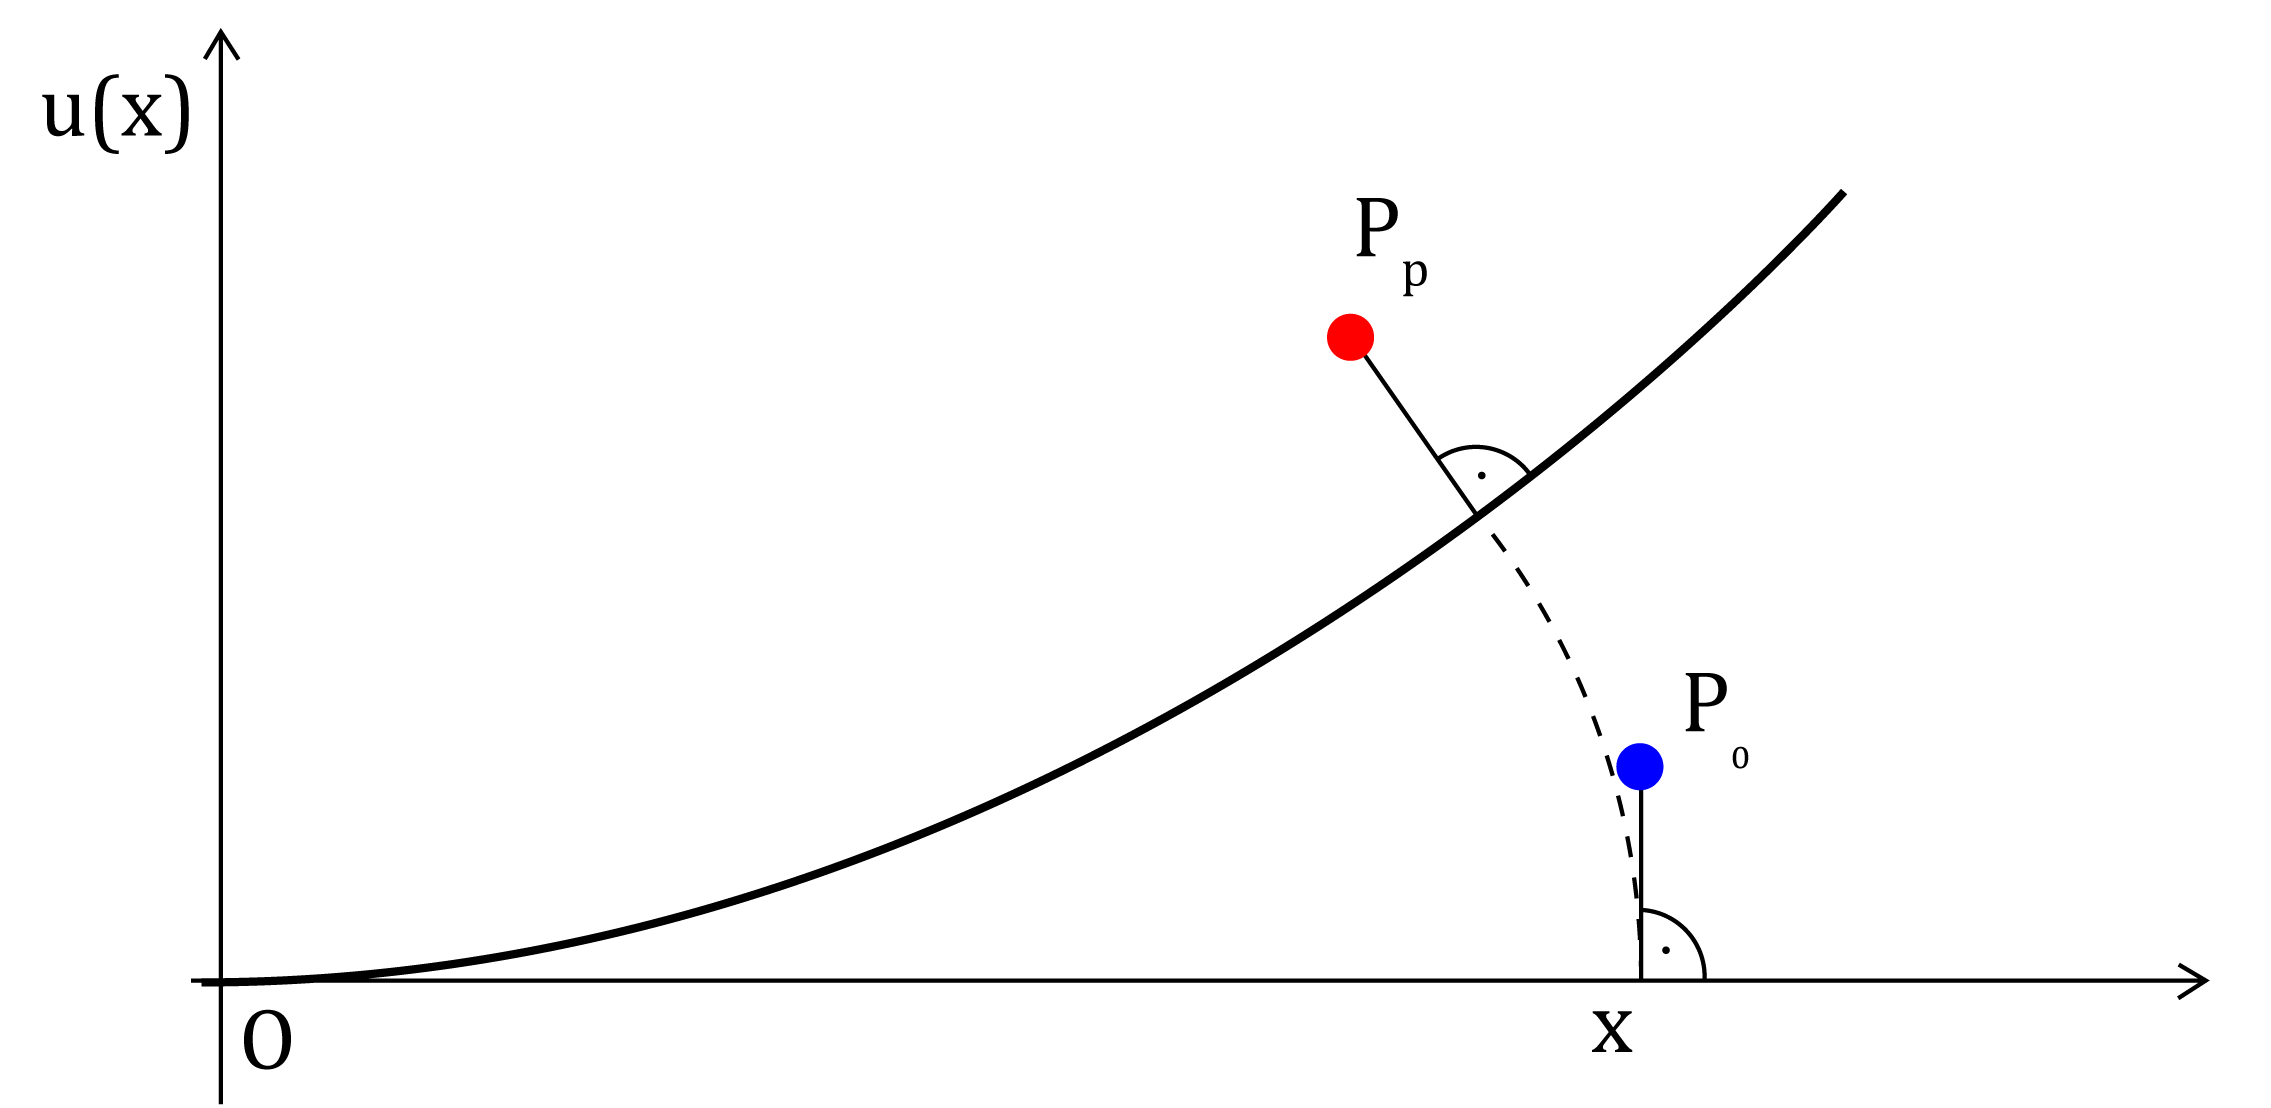
\includegraphics[width=0.5\textwidth]{./figures/revDef_ideal.png}
\caption{Myšlenkový model ohybu pomocí zpětné transformace\label{fig:bendModel}}
\end{center}
\end{figure}
 
Problém představuje určení parametru $x$ ohybové funkce $u(x)$ pro bod $P_p$ (deformovaný z $P_0$), který zmíněnou polohu na větvi definuje. Pro přesné určení je nutné zjistit nejbližší bod na ohybové funkci a pro ten pak zjistit jeho vzdálenost na křivce od počátku. 
\begin{figure}[!hbt]
\begin{center}
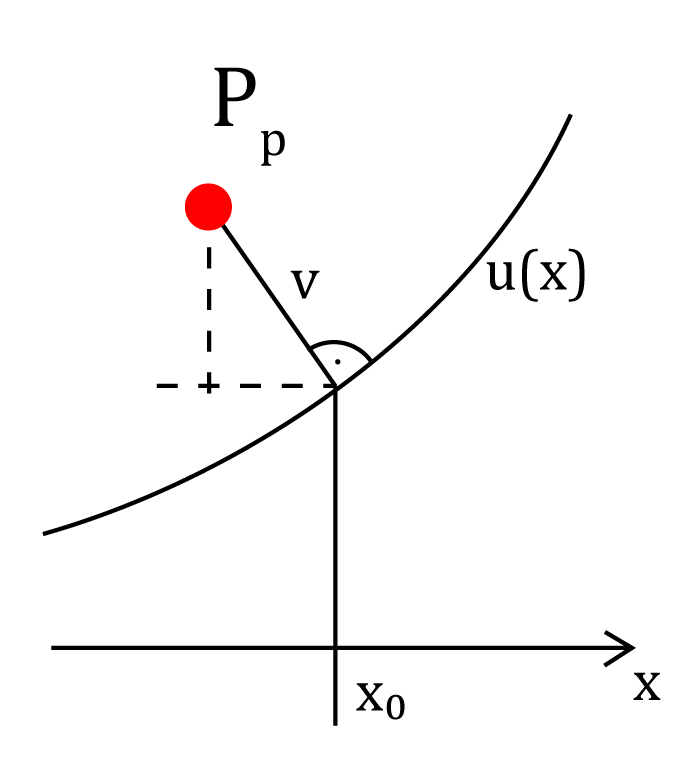
\includegraphics[width=0.25\textwidth]{./figures/revDef_dist.png}
\caption[Zjišťování nejbližšího bodu na ohybové křivce]%
{Zjišťování nejbližšího bodu na ohybové křivce $u(x)$\label{fig:closestPointOnCurve}}
\end{center}
\end{figure}

Bod $x_0$ lze určit z následujících rovnic, kde hledáme minimum pro vzdálenost $v$:

\begin{align}
\frac{\mathrm {d}{v}}{\mathrm {d}{x_0}} &= 0 \nonumber\\
v &= \sqrt{(x_0 - P_{px})^2 + (u(x_0) - P_{py})^2} \nonumber\\
\frac{\mathrm {d} \sqrt{(x_0 - P_{px})^2 + (c_2x_0^2 +c_4x_0^4 - P_{py})^2}}{\mathrm{d}x_0} &=0
\end{align}
Řešení je omezeno podmínkou:
\begin{align}
P_{px} \neq \pm \sqrt {\frac{-c_2 \pm \sqrt{c_2^2 - 4c_4P_{py}}}{2c_4}}
\end{align}

a transformuje se na problém hledání kořenů polynomu 7. stupně:

\begin{align}
\label{closestPointEq}
4c_4^2 x^7 + 6c_2c_4x^5 + (2c_2^2 - 4P_{py}c_4)x^3 + (1-2P_{py}c_2)x - P_{px} &= 0
\end{align}

Tento polynom nemá triviální řešení a může se stát, že řešení je i několik – což odpovídá situaci, kdy se více bodů z křivky deformuje do stejného místa (viz obrázek ~\ref{fig:multisolution} ).

Krom obtíží s řešením kořenů polynomu \eqref{closestPointEq} se tak přidává i určitá nejednoznačnost. Stále je však ještě potřeba vyřešit vzdálenost takto nalezeného bodu na ohybové křivce. Uvážíme-li, že takový složitý postup by se měl provádět pro každý zobrazovaný fragment textury, dostaneme se do patové situace.
\begin{figure}[here]%[!hbt]
\begin{center}
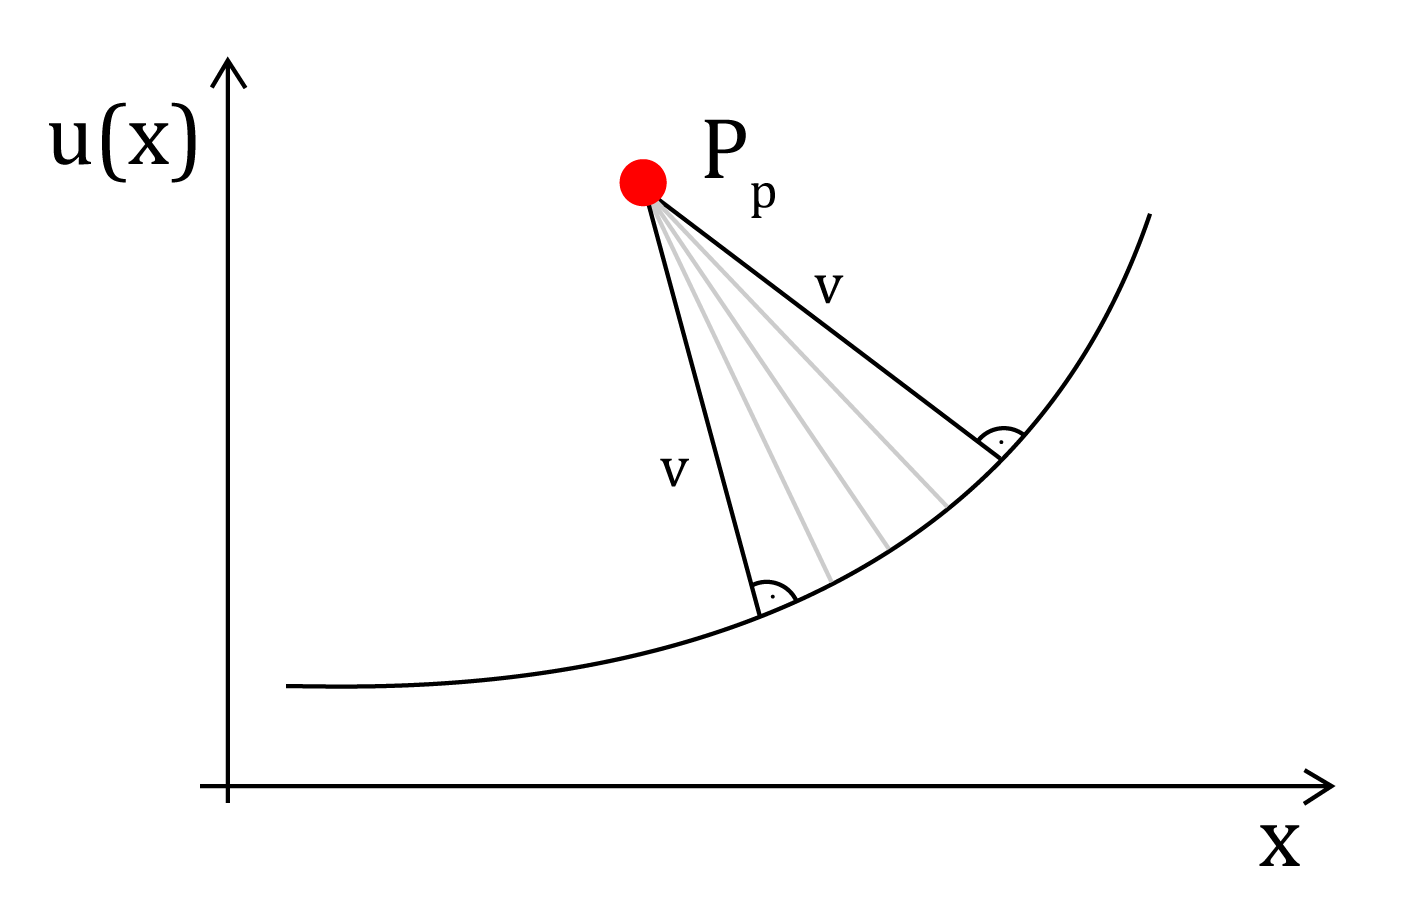
\includegraphics[width=0.5\textwidth]{./figures/revDef_multisolution.png}
\caption[Mnohoznačnost při zpětné transformaci]
{Znázornění problému mnohoznačnosti při určování, který bod je řídící pro zpětnou deformaci bodu $P_p$. U reálného stromu dojde v tomto případě ke kolizi takových větví.\label{fig:multisolution}}
\end{center}
\end{figure}
Zde je třeba rezignovat na dodržení shodného postupu jako v případě přímé deformace geometrie. Počáteční bod $O$ příslušné větve převedeme do souřadného systému textury ${S_p}$ a zjistíme projektovanou délku $L$ větve. {\bf Hledanou hodnotu x pak nahradíme vzdáleností $\left| OP \right|$, kterou normujeme délkou $L $ a omezíme na rozsah $\left \langle 0;1 \right \rangle$ }. Pro takovou hodnotu $x$ určíme deformační vektor $\vec{d}$ (posunutí bodu) a aplikujeme v opačném směru $\vec{-d}$ než při přímé transformaci.
 
\begin{figure}[!hbt]
\begin{center}
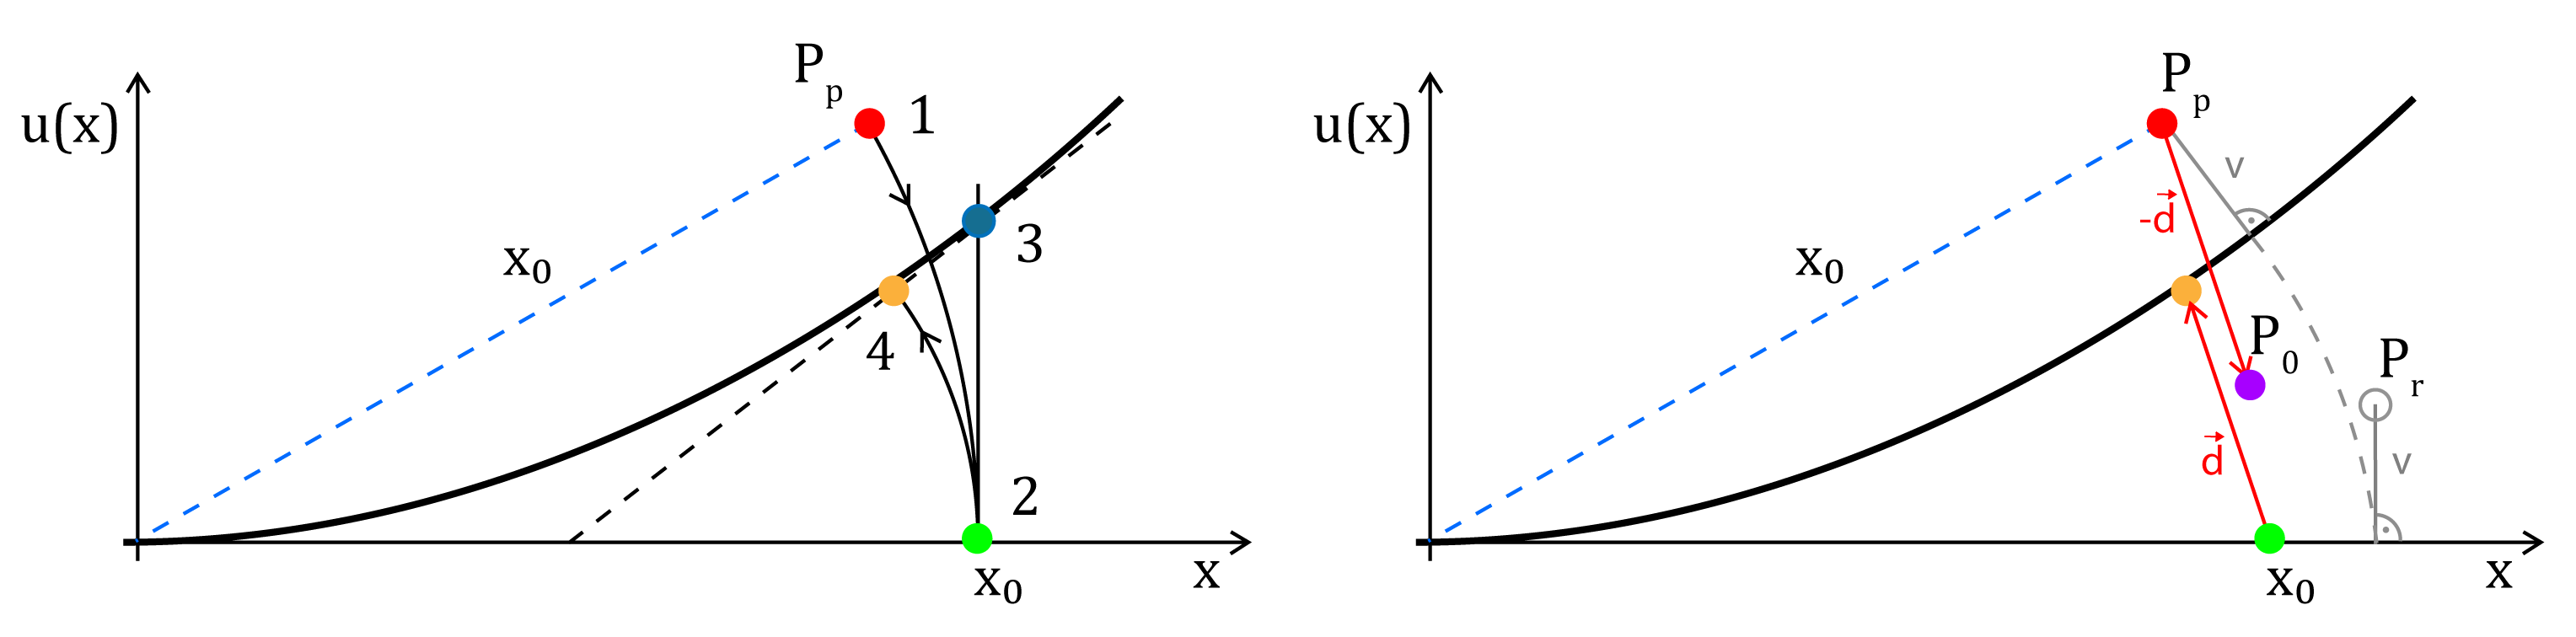
\includegraphics[width=1.0\textwidth]{./figures/revDef_process.png}
\caption[Postup zpětné transformace]
{Postup zpětné transformace: (vlevo) – postup určení deformace: Bod $P_p$ (1), pro který určujeme deformaci je ve vzdálenosti $x_0$ od počátku (2). Zjistíme hodnotu ohybové funkce v bodě $x_0$ (3). Provedeme korekci délky (4).
(vpravo) – určíme vektor posunutí $\vec{d}$ mezi body $x_0$ a (4) (v obrázku vlevo) odečtením od bodu $P_p$ se dostáváme na pozici předobrazu $P_0$. Šedivě je naznačen bod $P_r$, jež je skutečným předobrazem respektujeme-li myšlenkový model. \label{fig:backwardTransformationProcess}}
\end{center}
\end{figure}
\pagebreak
Je patrné, že chyba způsobená takovou hrubou aproximací $x_0$ je relativně malá pro body $P_p$, ležící přímo na ohybové křivce, ale roste tím víc, čím je od ní bod vzdálenější. Použitím vztahů \eqref{lengthCorrection} aplikovaným na projektované bázové vektory $\vec{r}_p$, $\vec{s}_p$ (zastoupené vektorem $\vec{b}_p$) dostaneme upravené vztahy pro korekce délky $\vec{c}_{\vec{b}}$, $\vec{c}_{\vec{b}}$.

\begin{align} 
\vec{c}_{\vec{b} }&= \vec{t} + \vec{b} \cdot f'_{\vec{b} } (x)\cdot\frac {d_{\vec{b} }(x)}{s_{\vec{b} }(x)}
 \end{align}

Deformaci v prostoru textury lze tedy popsat následovně:

\begin{align}
\label{backwardDeformation} 
\vec{P}_0 &= \vec{P}_p - \left ( u_{\vec{r}} (x) \cdot \vec{r}_p + u_{\vec{s}} (x) \cdot \vec{s}_p - \left (\vec{c}_{\vec{r}} +\vec{c}_{\vec{s}}  \right ) \right )
\end{align}


Zpětnou deformaci lze provádět i hierarchicky a to v pořadí od nejnižší úrovně větví v hierarchii až po kmen (tedy opačně, než v přímé transformaci). Je však nutné vyvážit náročnost takového postupu a jeho přidanou hodnotu. Například je možné deformaci provádět pro několik nejvyšších úrovní hierarchie. 
S opačným postupem tvorby hierarchické deformace v image-based modelu souvisí i problém správné aplikace směrové složky větru. Ve vztahu \eqref{windEq} je použit vektor $\vec{t}$ ovlivněný nadřazenými deformacemi. Ten však při opačném postupu zpětné deformace není znám. Předpokládáme-li provádění zpětné deformace pouze ve dvou úrovních (kmen + větve první úrovně) a rozumě malé výchylky, pak lze za vektor $\vec{t}$ dosadit nedeformovaný vektor $\vec{t}_p$, místo $\vec{W}$ použijeme $\vec{W}_p$ (směr větru v souřadné soustavě řezu). Vzniklá chyba není natolik vážná, aby představovala překážku u modelů s nižší percepční vahou, jakými nižší stupně LOD bezpochyby jsou.

Popsaná metoda má předpoklad dobře fungovat pro větve tvořící siluetu stromu v daném řezu. U takových větví se předpokládá, že jejich podélný vektor je zhruba rovnoběžný s rovinou řezu. Současně je třeba si uvědomit, že i fáze propagace dat má určitá omezení a funguje lépe pro siluetové větve. Jak se však ukazuje, právě tyto větve hrají největší roli při pozorování stromu s nižší percepční vahou. Hrají i podstatnou roli při přechodu mezi úrovněmi LOD.

Zbývá vyřešit pohyb jednotlivých listů. Pohybem větví nižších úrovní hierarchie a listů vzniká vysokofrekvenční šum v prostoru obrazu. Tento šum pozorovatel vnímá, ale nerozeznává již, jestli je způsoben pohybem větví, či samotných listů. Lze ho tedy napodobit použitím jediné deformace. Pro šum vyšších frekvencí je zároveň těžké rozlišit, zda jde čistě o pohyb, či jen změny barvy. Představíme-li si například, že list je zobrazen do jediného pixelu, pak pouhým natáčením listu zjevně měníme barvu zmíněného pixelu (barevný šum). Nerotační pohyb listu může způsobit obarvení jiného pixelu (pohybový šum). Pohyb listů může pak ústit v určité nepravidelné chvění elementárních fragmentů obrazu (případně větších oblastí – podle toho, kolik fragmentů zobrazuje stejný list).
\begin{figure}[!hbt]
\begin{center}
$\begin{array}{cc}
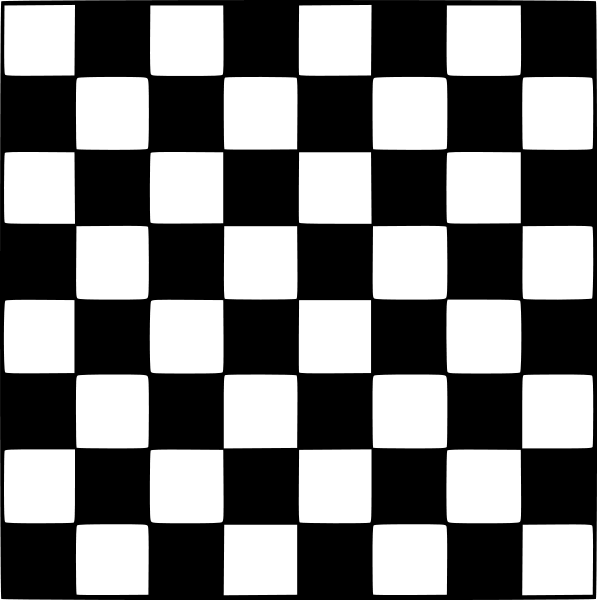
\includegraphics[width=0.35\textwidth]{./figures/distortion_before.png}&
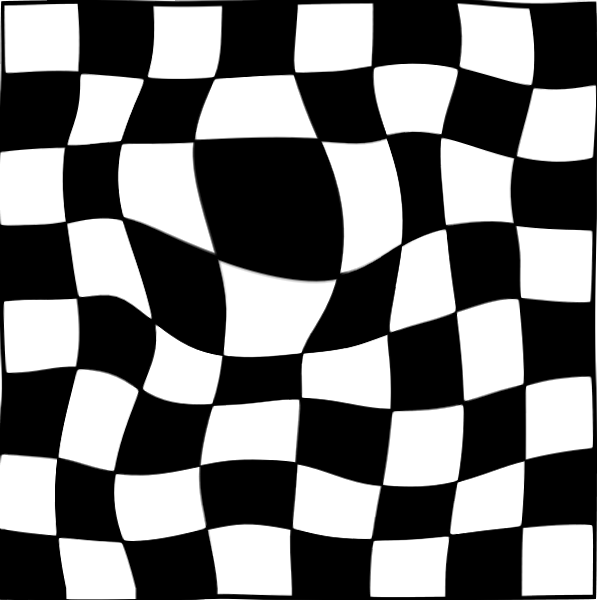
\includegraphics[width=0.35\textwidth]{./figures/distortion_after.png}\\
(a)&(b)
\end{array}$
\caption[Dvourozměrná deformace obrazu]
{Příklad dvourozměrné deformace obrazu technikou displacement-mappingu. Originál $(a)$ a deformovaný obraz $(b).$\label{fig:distortion}}
\end{center}
\end{figure}
\pagebreak
Pohybovou složku šumu lze vcelku dobře napodobit metodou zvanou {\bf displacement-mapping}. V základní verzi získává z řídící textury informace o posunutí v prostoru deformovaného obrazu – v tomto případě barevné textury. Vhodnými změnami řídící textury (posun souřadnic, kombinace různých textur) lze plynule deformovat výsledný obraz. 

Šumový displacement-mapping je možné zapsat například takto:
\begin{align} 
color &= T_{color}(T_{def}(\vec{o}_t + t \cdot \vec{d}_1)+T_{def}(\vec{o}_t + t \cdot \vec{d}_2)),
\end{align}
kde $T_{def}(\vec{x})$ je texturovací funkce, jež zobrazuje souřadnice $\vec{x}$ na jiné, a $T_{color}(\vec{x})$ přiřazuje daným souřadnicím $\vec{x}$ barvu. Jak je patrné, deformace závisí na obsahu deformační textury. Pokud bude obsahovat jen plynulé přechody, bude i deformace spojitá.



Barevnou složku šumu je možné vytvořit například tak, že pro každý zobrazený list v řezu měníme jeho natočení ke světlu (normálu) a následně provádíme standardní vyhodnocení Phongova osvětlovacího modelu. Je tedy nezbytné, aby tato transformace normál proběhla pro konkrétní list koherentně - nejlépe stejně. V opačném případě by mohl výsledný šum mít mnohem vyšší frekvenci, než by bylo vhodné.
\newpage

\subsection{Řízení úrovně detailu}
\label{sec-LODcontrol}
V předchozích kapitolách jsou navrženy metody, jak zobrazovat vegetaci (stromy) ve třech různých stupních detailu. Nejvyšší (označme ji \emph{LOD\_0}) využívá podrobné geometrické reprezentace a poskytuje nejlepší kvalitu zobrazení pro pohledy zblízka. Přesvědčivě tak lze zobrazit i jednotlivé pohybující se listy stromu. LOD\_0 je však vcelku náročná na výkon a není možné ji uplatnit plošně na všechny stromy rozsáhlé lesní scény. Pro stromy s nižší percepční vahou (není třeba je zobrazovat tak podrobně) byly navrženy image-based metody (označme LOD\_1 a LOD\_2). Ty poskytují sice nižší kvalitu zobrazení (na úrovni zobrazení a pohybu celého stromu), ale jsou méně náročné na výkon. 
\begin{figure}[!h]
\begin{center}
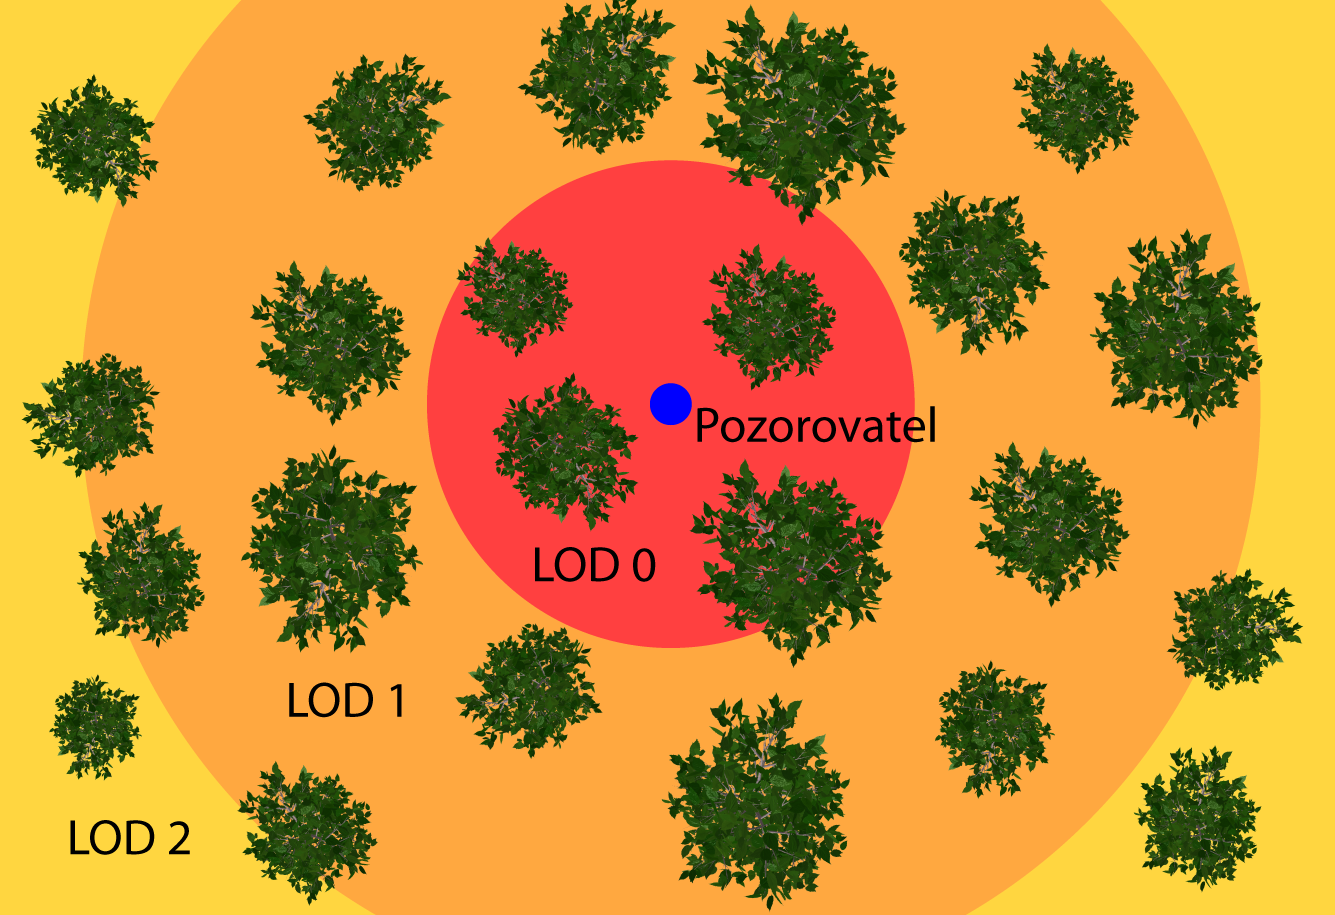
\includegraphics[width=0.75\textwidth]{./figures/LODcontrol.png}
\caption{Znázornění zón, kde se instance stromů vykreslují danou metodou.\label{fig:lodZones}}
\end{center}
\end{figure}

Pro určení přibližné percepční váhy se běžně využívá vzdálenostní kritérium. Blízké stromy v okolí pozorovatele jsou tedy zobrazeny metodou LOD\_0, od určité vzdálenosti $v_1$ se využívá metody LOD\_1 a obdobně pro vzdálenost $v_2$ a metodu LOD\_2, přičemž platí, že $0<v_1<v_2$ .

Jedná se tedy o diskrétní třístupňový LOD systém. Určení vzdálenosti k jednotlivým instancím stromu lze provádět buď v prostoru (vhodné např. aplikace typu letecký simulátor), nebo pouze v horizontální rovině (aplikace s pohledem omezeným na pohled z okolí úrovně terénu). Vzdálenosti $v_1$ a $v_2$ je třeba přizpůsobit konkrétním modelům vegetace a scéně obecně, stejně jako optimalizaci z hlediska výkonu, na který mají podstatný vliv.


\subsection{Přechody mezi úrovněmi detailu}
\label{sec-LODtransitions}
Kvalitu metody vytvoření a řízení LOD lze posuzovat jak z hlediska optimalizace výkonu, tak i podle toho, nakolik si je pozorovatel vědomý, že k nějaké optimalizaci vůbec dochází. Bohužel, jak již bylo v předchozím textu naznačeno, diskrétní metody LOD se mohou potýkat s nežádoucím jevem zvaným LOD-popping, který prozrazuje, že se scéna mění, aniž k tomu je z hlediska pozorovatele zřejmý důvod. Nejnaivnějším způsobem jak přecházet mezi úrovněmi detailu je skokové přepnutí. Právě skoková změna na sebe poutá pozornost a tak nejde o dobré řešní. Vhodnější je jednotlivé úrovně plynule prolnout. Toho lze docílit buď technikou zvanou \emph{morphing}, která plynule převádí tvar jednoho tělesa na druhé transformací geometrie, nebo prostým prolnutím výsledných obrazu díky řízení průhlednosti. Ukazuje se však, že přístup známý jako \emph{cross-fade} může vytvářet určité nechtěné problémy. 



